\documentclass[a4paper]{article}

\usepackage[english]{babel}
\usepackage[utf8]{inputenc}
\usepackage{fullpage}
\usepackage{amsmath}
\usepackage{graphicx}
\usepackage[colorinlistoftodos]{todonotes}
%\usepackage{hyperref}
\usepackage{amssymb}
\usepackage{subfigure}
\usepackage{url}
\usepackage[pagebackref=true,colorlinks,linkcolor=red,citecolor=green,breaklinks=true,bookmarks=false]{hyperref}
\usepackage{outline} 
\usepackage{pmgraph} \usepackage[normalem]{ulem}
\usepackage{graphicx} \usepackage{verbatim}
\usepackage{indentfirst}
\setlength{\parindent}{2em}
% \usepackage{minted} % need `-shell-escape' argument for local compile

\title{
    \vspace*{1in}
    
\includegraphics[width=2.75in]{figures/zhenglab-logo} \\
    \vspace*{1.2in}
    \textbf{\huge Introduction to Deep Learning}
    \vspace{0.2in}
}

\author{Hongzhi Liu \\
    \vspace*{0.5in} \\
    \textbf{VISION@OUC} \\
    \vspace*{1in}
}

\date{\today}


\begin{document}
\par
\maketitle
\setcounter{page}{0}
\thispagestyle{empty}
\newpage


\section{Concept of Neural Network}

Thanks to Coursera and NetEase online courses, I can get access to Andrew Ng's deep learning class which includes five segments in the whole specialization \cite{course1,course2}. According to the teaching plan, I will learn about introduction to deep learning as the first week learning tasks.

Deep Learning refers to training neural networks, as Andrew Ng says, having a lot of practical value during our daily life such as predicting housing price. So the class begins with concept explanation of neural network. 

\subsection{A Simple Neural Network}
First, I have learnt a very simple neural network of housing price prediction. Supposing we have a data sets with six houses that size and price of the house as shown in Fig.~\ref{p1}\subref{p1a}, we will be able to fit a function to predict the price of houses which is the function of the size. Then with linear regression, Andrew Ng puts a straight line to these data and we get a straight line as shown in Fig.~\ref{p1}\subref{p1b}. But actually prices can never be negative, so instead of the straight line fit which eventually will become negative, we bend the curve near x axis above. The thick blue line we got ends up being our function for predicting the price of houses as a function of this size.

With the function for house price prediction and a straight line below in Fig.~\ref{p1}, we can get a very simple neural network as shown in Fig.~\ref{p2}\subref{p1a}.
\begin{figure}[b] 
	\centering 
	\subfigure[]{ 
		\label{p1a} %% label for first subfigure 
		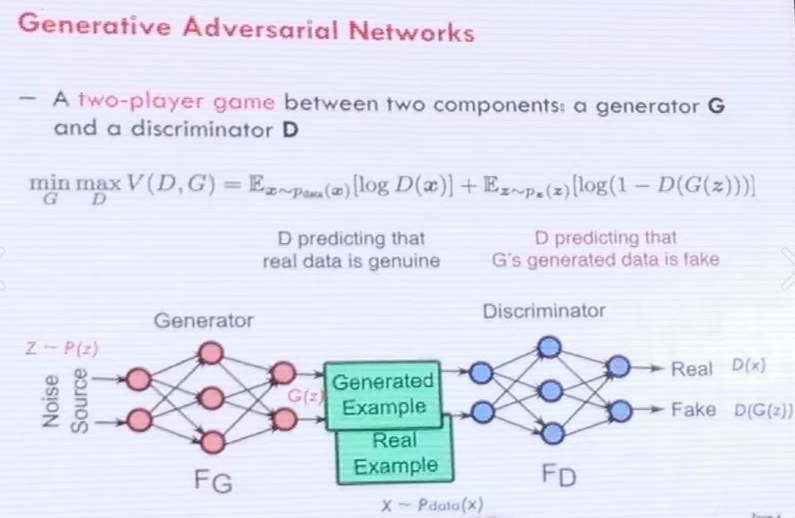
\includegraphics[scale=0.3]{figures/2.png} 
	} 
	\subfigure[]{ 
		\label{p1b} %% label for second subfigure 
		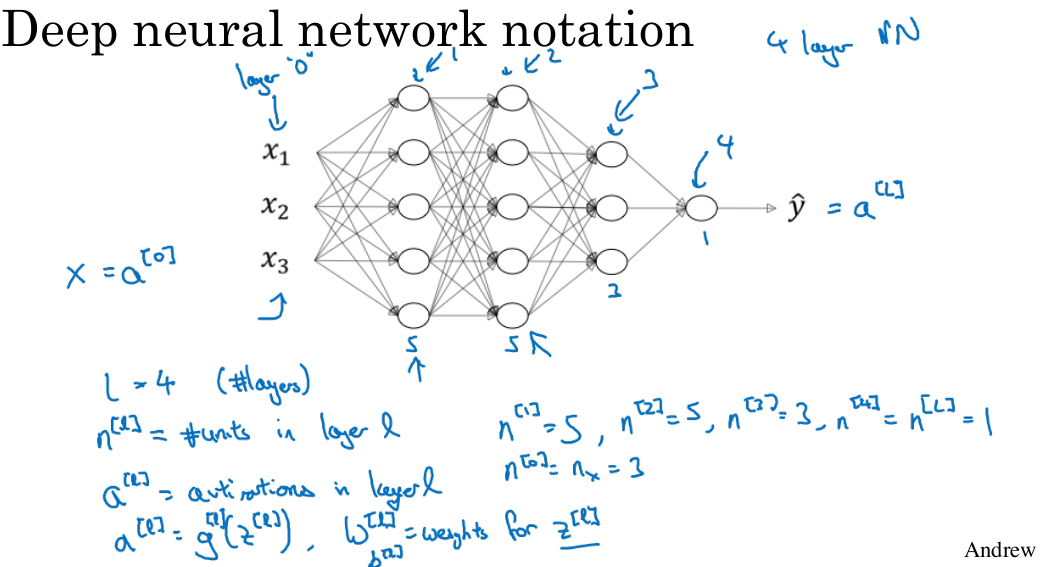
\includegraphics[scale=0.3]{figures/1.png} 
	} 
	\caption{Housing price prediction} 
	\label{p1} %% label for entire figure 
\end{figure}

\begin{figure}
	\centering 
	\subfigure[]{ 
		\label{p2a} %% label for first subfigure 
		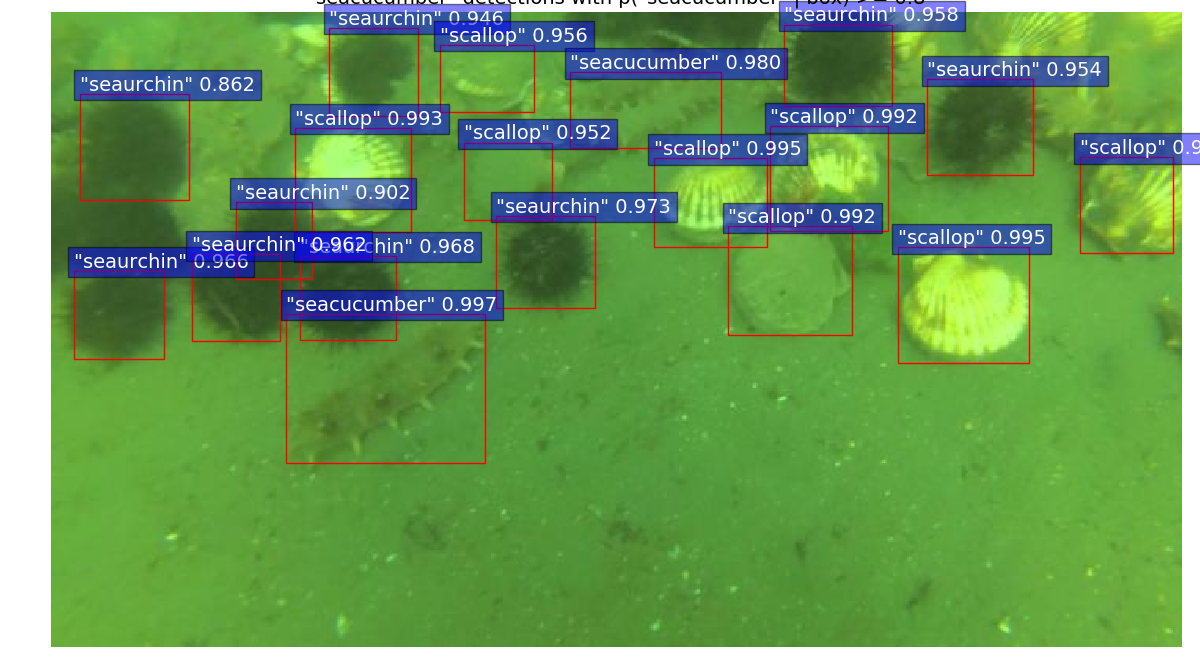
\includegraphics[scale=0.2]{figures/3.png} 
	} 
	\subfigure[]{ 
		\label{p2b}
		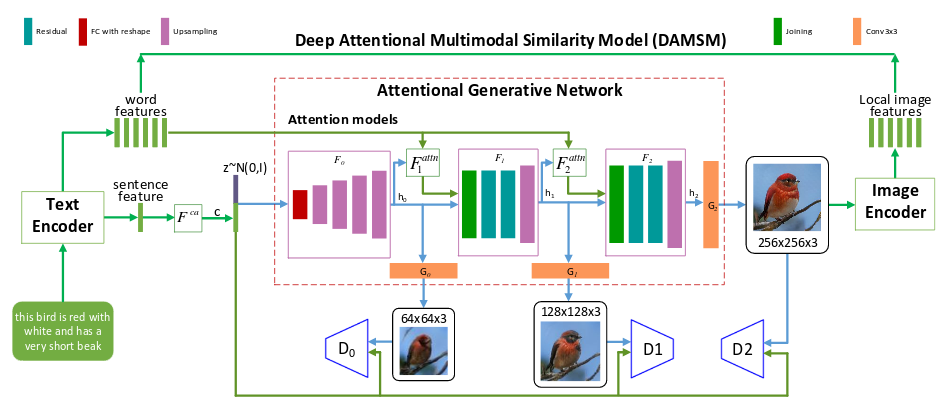
\includegraphics[width=.35\textwidth]{figures/4.png} 
	}
	\subfigure[]{ 
		\label{p2c}
		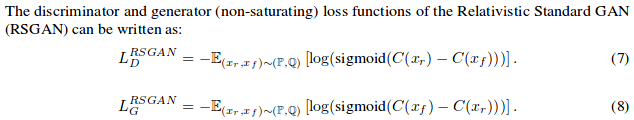
\includegraphics[width=.35\textwidth]{figures/5.png} 
	} 
	\caption{We have as the input to the neural network that the size of a house which one we call x and then it outputs the price which we call y. The little circle, which is a single neuron in a neural network, implements this function that we drew above. } 
	\label{p2} 
\end{figure}

The function about the price of houses prediction is called a ReLU function which stands for rectified linear units. And rectify just means taking a max of 0 which is why you get a function shape as shown in Fig.~\ref{p1}. 

\subsection{A Basic Neural Network Application}
Knowing a simple neural network example, I will be able to learn a more confuse one. As is known to all, instead of predicting the price of a house just from the size, we can have some other features such as the number of bedrooms, zip codes and wealth just as shown in Fig.~\ref{p2}\subref{p1b}. We might think that one of these things really affects the price of a house is family size. So we can measure a house whether fit a family of three, four or even five. Besides, the zip code maybe as a future to tell us walkability that just walks to the grocery store or school. Furthermore, the zip code as well as the wealth maybe tells us how good the school quality is. So each of these little circles can be one of those ReLUs. 

Based on the size and number of bedrooms, we can estimate the family size. And based on walkability, zip code and wealth, we can estimate the school quality. Then finally we might know the way people decide how much they will pay for a house, which really matter to people. So x is all of these four inputs in this example, y is the housing price we try to predict in Fig.~\ref{p2}\subref{p2c}.

Now let me briefly summarize this example of housing price prediction which is a basic neural network application. Given these input features, the neural network mentioned above will be to predict the price y. We can know layer with features is the input layer. Besides, the layer in the middle of the neural network are density connected, because every input feature is connected to every one of those circles in the middle. And the remarkable thing about neural networks is that given enough data about x and y. Training examples with both x and y, neural networks are remarkably good at figuring out functions that accurately map from x to y. 

\section{Supervised Learning with Neural Networks}

Recently, almost all the economic value created by neural networks has been through one type of machine learning, called supervised learning. In supervised learning, we have some input x and we want to learn a function mapping to some output y. Just like the housing price prediction application where we input some features of a home and try to output or estimate the price y. Here are some examples of supervised learning as shown in Tab.~\ref{t1}.
\begin{table}
	\centering
	\begin{tabular}{c|c|c}
			\hline
			Input(x) & Output(y) &Application  \\
			\hline
			Home features & Price &Real estate\\
			Ad, user info & Click on ad? (0/1) &Online advertising  \\
			Image & Object(1,$\ldots$,1,000) &Photo tagging   \\
			Audio & Text transcript &Speech recognition  \\
			English & Chinese &Machine translation  \\
			Image, Radar info & Position of other cars &Autonomous driving  \\
			\hline
	\end{tabular}
	\caption{Neural networks application}
	\label{t1}
\end{table}

\subsection{Supervised Learning Application}
Possibly the single most lucrative application is online advertising. By inputting information about an ad. to the website, it's thinking of showing us and some information about the user. Neural networks have gotten very good at predicting whether or not people click on an ad. 

\begin{figure}
	\begin{center}
		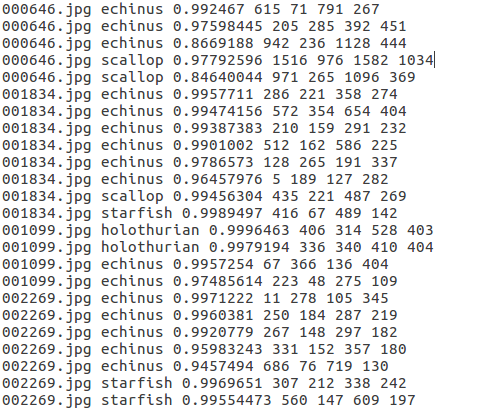
\includegraphics[scale=0.4]{figures/7.png}
	\end{center}
	\caption{Neural networks examples.}
	\label{p3}
\end{figure}

Computer vision has also made huge strides in the last several years, mostly due to deep learning. So we might input an image and want to output an index, say from 1 to 1,000 trying to tell you if this picture might be any one of 1,000 different images. I think the recent progress in speech recognition has also been very exciting, where we can now input an audio clip to a neural network, and have it output a text transcript. Machine translation has also made huge strides thanks to deep learning where now we can have a neural network input an English sentence and directly output a Chinese sentence. And in autonomous driving, we might input an image which is a picture of what's in front of the car as well as some information from a radar. Only if based on that, a neural network can be trained to tell us the position of other cars on the road.
\begin{figure} 
	\centering 
	\subfigure[]{ 
		\label{p4a} 
		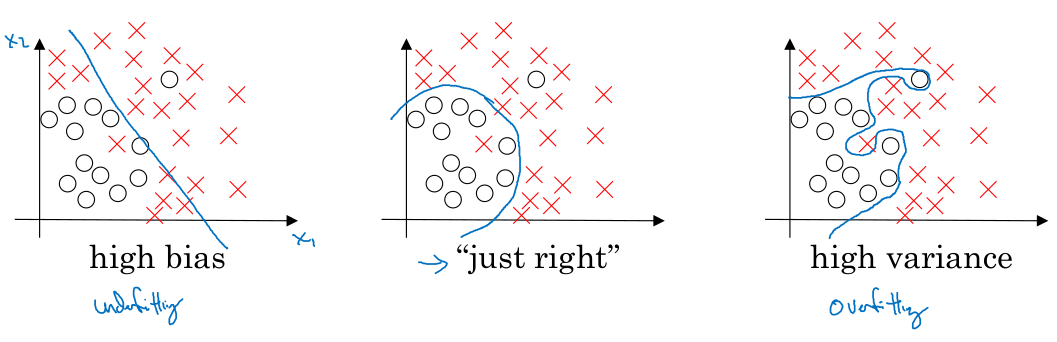
\includegraphics[scale=0.35]{figures/8.png} 
	} 
	\subfigure[]{ 
		\label{p4b}
		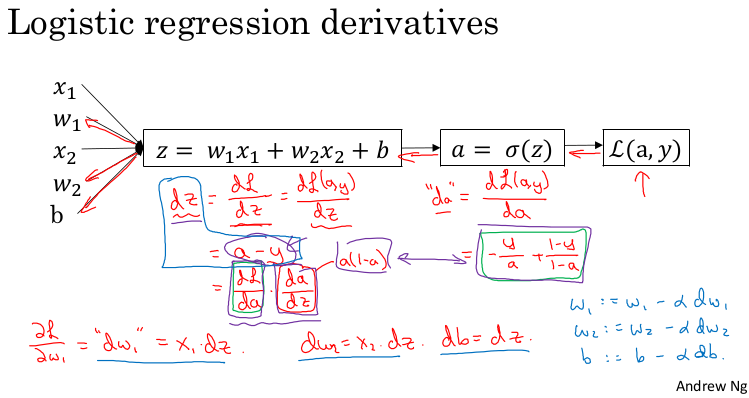
\includegraphics[scale=0.35]{figures/9.png} 
	} 
	\caption{Structured and unstructured data} 
	\label{p4} 
\end{figure}

In the real estate and online advertising application that we learn in the last section, we use a universally standard neural network architecture as the left network in Fig.~\ref{p3}. For image applications we'll often use convolution on neural networks, often abbreviated CNN as the middle network in Fig.~\ref{p3}. And as to sequence data such as audio and language, we often use an RNN, a recurrent neural network for these applications.
\begin{figure}
	\begin{center}
		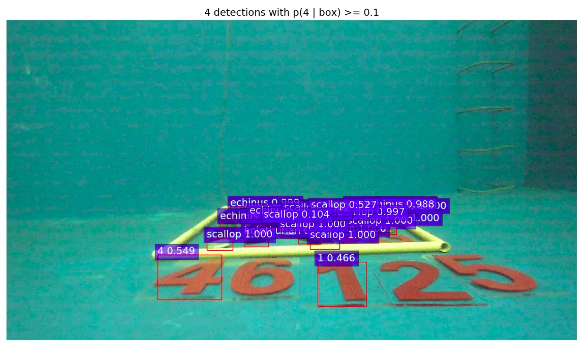
\includegraphics[scale=0.4]{figures/10.png}
	\end{center}
	\caption{Scale drives deep learning progress. On the horizontal axis in figure, we plot the amount of data for a task and on the vertical axis we plot the performance on above.}
	\label{p5}
\end{figure}.

\subsection{Structured and Unstructured Data}
I have also learnt about applications of machine learning to both Structured Data and Unstructured Data as shown in Fig.~\ref{p4}. In housing price prediction, we have a database or the column that tells people the size and the number of bedrooms which is structured data just like Fig.~\ref{p4}\subref{p4a}. Besides, in predicting whether or not a user will click on an ad, we might have information about the user such as the age, some information about the ad and then labels we're trying to predict. So that's structured data, meaning that each of the features has a very well defined meaning. In contrast, unstructured data refers to things like audio or images where ones might want to recognize what in the image or text is just like Fig.~\ref{p4}\subref{p4b}.

Furthermore, one of the most exciting things about the rise of neural networks is that, with deep learning and neural networks, computers are now much better at interpreting unstructured data as well compared to just a few years ago.  And this creates opportunities for many new exciting applications that use speech recognition, image recognition, natural language and processing on text.

\section{Deep Learning is Taking off}

In this section, I learn about reason why deep learning is now taking off. We often say that scale has been driving deep learning progress. If we plot the performance of a traditional learning algorithm as a function of the amount of data, we have might get a curve where the performance improves for a while as we add more data but after a while, the performance pretty much plateaus right. Suppose our horizontal lines enjoy that very well, people understand was that it didn't know what to do with huge amounts of data and what happened in our society over the last 10 years.

Thanks to the digitization of society and the rise of inexpensive cameras built into our cell phones, we have been collecting more and more data over the last 20 years for a lot of applications. The networks turns out that if we train a small neural net then performance maybe looks like the yellow line in Fig.~\ref{p5}. And if we train a somewhat larger Internet that's called as a medium-sized internet, something is a little bit better. And if we train a very large neural net then it often just keeps getting better and better.
\begin{figure}[b]
	\begin{center}
		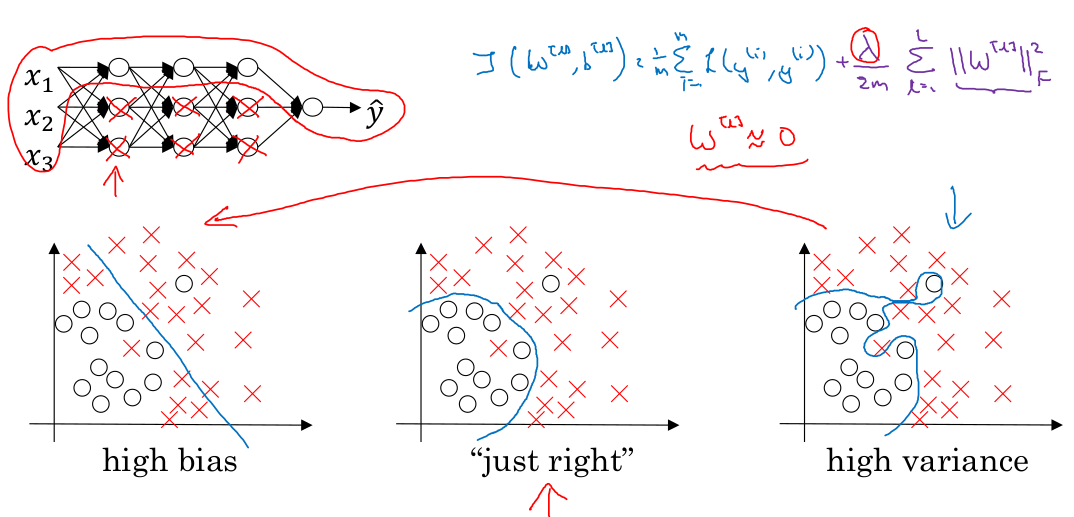
\includegraphics[scale=0.4]{figures/11.png}
	\end{center}
	\caption{Scale drives deep learning progress.}
	\label{p6}
\end{figure}.

So we often say that scale has been driving deep learning progress. And by scale Andrew Ng means both the size of the neural network we need just a neural network with a lot of hidden units, parameters and connections as well as scale of the data. In modern rise of deep learning, it was scaled data and scale of computation just our ability to train very large networks either on a CPU or GPU that enabled us to make a lot of progress in the early days. Besides, increasingly in the last several years we've seen tremendous algorithmic innovation as well. 

The reason that fast computation is important is that it turns out the process of training our network. This is very intuitive when we have an idea for a neural network architecture and then we implement our idea and code implementing the idea. Then we run an experiment which tells how well the neural network does. And by looking at it, we go back to change the details of new network and go around this circle over and over as shown in Fig.~\ref{p6}. Besides, when the neural network takes a long time to train, it just takes a long time to go around the cycle. And there's a huge difference in our productivity building effective neural networks when we can have an idea and try it.

In fact, faster computation has really helped in terms of speeding up the rate at which we can get an experimental result back. This has really helped both practitioners of neuro networks as well as researchers working and deep learning iterate much faster and improve our ideas much faster. So all this has also been a huge boon to the entire deep learning research community.

% If you don't cite any references, please comment the following two lines
\bibliographystyle{ieee}
\bibliography{ref.bib}

\end{document}